\documentclass[DIV=14]{scrartcl}
\usepackage[utf8]{inputenc}
\usepackage[T1]{fontenc}  % needed for the correct underscores in \texttt
\usepackage{graphicx}
\usepackage{amsmath}
\usepackage{physics}

\usepackage{siunitx}
\DeclareSIUnit{\LSB}{LSB}

\usepackage{hyperref}
\hypersetup{pdfborder = 0 0 0}  % links without decoration

\usepackage{censor}
\usepackage{amssymb} % just for the sample report, no use in a real report

\titlehead{
    Laboratory for Electrical Instrumentation and Embedded Systems \\
    IMTEK -- Department of Microsystems Engineering \\
    University of Freiburg \vspace{0.5cm} \\
    Sensors Lab Course \\
    Winter term 2022/23 \vspace{1.5cm}}

\title{Lab Report M2}
\subtitle{Magnetic Sensor}
\author{Rafael Andrioli Bauer (5163344)}

\begin{document}
    \maketitle

    \thispagestyle{empty}

    \vfill
    \begin{center}
        
\includegraphics{ufcd-logo-e1-a4-color.pdf} \vspace{1cm} \\
    \end{center}
    \vfill

    \clearpage


    \section{Introduction}

    The Earth's magnetic field is a complex phenomenon that has been studied for centuries.
    It is generated by the movement of molten iron in the Earth's core, and it plays an important role in
    protecting the Earth's surface from harmful solar radiation and charged particles~\cite{labManual}.
    In this module, the Earth's magnetic field was measured using a magnetic sensor present
    in the Nicla Sense ME Board.
    Properties of the sensor BMM150 are also investigated.
    To conclude, the accuracy of the results are discussed.



    \section{Theory}\label{sec:theory}

    The Earth's magnetic field is a three-dimensional vector field that can be represented by its horizontal and vertical components~\cite{labManual}.
    The horizontal component, also known as the horizontal magnetic field (Equation~\ref{eq:Bhorizontal}), is the component of the magnetic field
    that lies in the earth's surface plane and is defined by the $x$ and $y$-axis.
    The vertical component, also known as the vertical magnetic field (Equation~\ref{eq:Bvertical}), is the component of
    the magnetic field that is perpendicular to the earth's surface and is defined by the $z$-axis~\cite{labManual}.

    \begin{subequations}
        \begin{alignat}{1}
            & B_{\mathrm{hor}} = \sqrt{B_{\mathrm{x}^2} + B_{\mathrm{y}}^2} \label{eq:Bhorizontal}\\
            & B_{\mathrm{vert}} = B_{\mathrm{z}} \label{eq:Bvertical}\\
            & B = \sqrt{B_{\mathrm{x}^2} + B_{\mathrm{y}}^2 + B_{\mathrm{z}}^2}  \label{eq:Btotal}
        \end{alignat}
    \end{subequations}

    The decomposition of the magnetic field into horizontal and vertical components is useful because it
    allows for a more detailed understanding of the Earth's magnetic field.
    When the horizontal component of the magnetic field is measured, it is possible to determine the direction of
    magnetic north, which is the direction of the horizontal component.
    However, this direction may not align with true north, which is the direction of the geographic North Pole~\cite{CartographersOffice}.
    The angle between these two directions is known as magnetic declination ($\delta_B$), illustrated in Figure~\ref{fig:magneticDeclination}.

    \begin{figure}[!h]
        \centering
        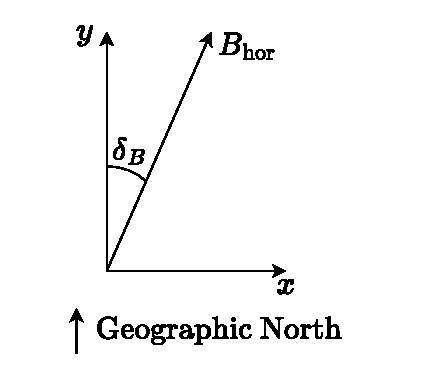
\includegraphics[width=.4\textwidth]{figures/MagneticDeclination}
        \caption{Illustration of magnetic declination (author's own work).}
        \label{fig:magneticDeclination}
    \end{figure}

    It can be computed using Equation~\ref{eq:magneticDeclination}.

    \begin{equation}
        \delta_B = \arctan{\frac{B_{\mathrm{y}}}{B_{\mathrm{x}}}}
        \label{eq:magneticDeclination}
    \end{equation}

    \subsection{Magnetic Sensor}\label{subsec:magnetic-sensor}

    Arduino Nicla has the barometric sensor BMM150, from Bosch Sensortech.
    It is a high-performance, low-power, triaxial geomagnetic sensor in which uses
    a Hall Effect technology that allows to measure magnetic fields with a high resolution and a wide measurement range~\cite{BMM150}.

    The Hall effect is a phenomenon that occurs when a conductor carrying current
    is placed in a magnetic field, which causes a voltage to be generated perpendicular to the current and the magnetic field~\cite{labManual}.
    The basic setup is illustrated in Figure~\ref{fig:hallEffect}

    \begin{figure}[!h]
        \centering
        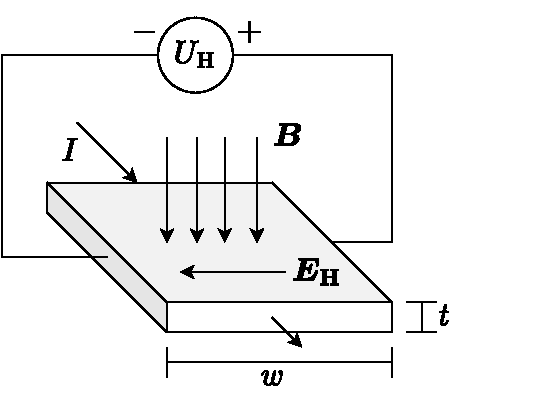
\includegraphics[width=.3\textwidth]{figures/HallEffect}
        \caption{Principle of hall efect. Current flowing through conductor under a magnetic field $B$(adapted from~\cite{labManual}).}
        \label{fig:hallEffect}
    \end{figure}

    When a current $I$ flows through a conductor, it causes a flow of electrons $e$ with velocity $v$ through the material.
    When this conductor is placed in a magnetic field $\boldsymbol{B}$, the electrons are deflected due to the interaction with the field
    and establish an electric field  $\boldsymbol{E_{\mathrm{H}}}$ which causes an electric force balancing ou the
    \textit{Lorentz Force}~\cite{labManual}.
    The equation describing it is the following:

    \begin{equation}
        e\boldsymbol{E_{\mathrm{H}}} = -e\boldsymbol{v} \times \boldsymbol{B}
        \label{eq:forceBalances}
    \end{equation}

    This results in a voltage difference across the conductor.
    This voltage difference is known as the Hall voltage $U_H$, and it is proportional to the magnetic field
    strength, the current, and the properties of the conductor, such as its width $w$ and thickness $t$.
    It can be expressed as:
    \begin{equation}
        U_H = -wvB
        \label{eq:hallVoltageWidht}
    \end{equation}
    or
    \begin{equation}
        U_H = -\frac{IB}{ent}
        \label{eq:hallVoltageCurrent}
    \end{equation}
    where $n$ is the charge carrier density~\cite{labManual}.

    \subsubsection{FlipCore}\label{subsubsec:flipcore}
    Bosch Sensortec's FlipCore technology shares similarities in its operating principle with that of a fluxgate sensor~\cite{labManual}.
    However, the FlipCore element has a simpler design, measurement process, and also consumes less power
    and generates less noise than a Hall sensor~\cite{labManual}.

    The fluxgate is made up of an easily saturable ferromagnetic material core, which is wound with two coils;
    an excitation coil, and a sense coil~\cite{fluxGate}.
    Figure~\ref{fig:fluxGate} depicts the ring core design of the fluxgate.

    \begin{figure}[hbt!]
        \centering
        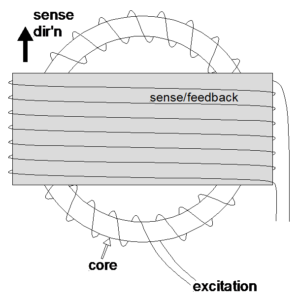
\includegraphics[width=.4\textwidth]{figures/fluxgate}
        \caption{Fluxgate sensor setup~\cite{flixGateImage}.}
        \label{fig:fluxGate}
    \end{figure}

    The excitation coil magnetizes its core while the sense coil reads the induced signal.
    Whenever an external magnetic field superimposes the induced magnetic field, it causes a signal detected as
    a 2nd harmonic~\cite{labManual}.



    \section{Methods}\label{sec:methods}
    A battery-powered notebook was used to take all measurements from an Arduino Nicla Sense Board ME containing a BHI260AP.
    It was connected to the computer via USB.
    The same notebook was used as a power supply for the board as well as a data logger.
    The board was programmed using the Arduino IDE 2.0.2 with the \texttt{Arduino\_BHY2} library version 1.0.5 (Bosch Sensortec).
    A small MATLAB application called \textit{SampleNicla} was developed to log the data.
    MATLAB was also used to process the data.
    The source code is available in \href{https://github.com/RafasLectures/sensorslab/blob/main/SampleNicla.mlapp}{GitHub}
    (\texttt{https://github.com/RafasLectures/sensorslab/})

    In a \SI{10}{\hertz} sampling rate (every \SI{100}{\milli\second}), the Arduino program reads the magnetometer
    virtual sensors \texttt{SENSOR\_ID\_MAG\_PASS} from the BMM150.
    The sensitivity of the sensor was the default \SI{16}{\LSB\per\micro\tesla} for all three axis~\cite{BMM150}.

    In Task~1 1000 measurements were taken in my house at a flat surface according to the setup shown Figure~\ref{fig:setup}
    at a temperature of 18ºC.
    Task~2, 3, 4 and 5, 100 measurements were performed in front of the building 52 in the street that
    points to the geographic north at a temperature of 15ºC.

    For all tasks the sensor was placed in a flat surface with its $z$-axis pointing upwards (Figure~\ref{fig:setup}).
    The $z$ direction on the sketch maps to the one displayed in the Arduino board instead of the one from~\cite{BMM150}.
    It seems that the axis of BMM150 were remapped by the framework used in Arduino to use the same coordinate system
    as the other sensors on the board ($z$ pointing upwards), such as accelerometer and gyroscope.
    The axis of BMM150 can be remapped via an API~\cite{BMM150}.

    On Task 2 the offset of every axis of the sensor was computed.
    In order to measure the offset two other setups in a flat surface were done:
    one with the $x$ and $y$-axis were flipped by 180º in relation to Figure~\ref{fig:setup}, and
    another where $x$ and $z$-axis were flipped by 180º in relation to Figure~\ref{fig:setup}.

    Assuming the sensor has an offset, we can say that the measured value is
    \begin{equation}
        U_{\mathrm{measured}} = U_{\mathrm{offset}} + U_{\mathrm{real}}
        \label{eq:measuredValue}
    \end{equation}

    If we have a constant magnetic field $\boldsymbol{B}$ and we flip the axis by 180º, we assume that $U_{\mathrm{real}}$ will
    have an inverted signal.

    Let $U_1$ and $U_2$ be two different measurements, where $U_1$ is non-inverted axis and $U_2$ has the axis inverted by 180º.
    Then we can write
    \begin{subequations}
        \begin{alignat}{1}
            & U_{1} = U_{\mathrm{offset}} + U_{\mathrm{real}}\\
            & U_{2} = U_{\mathrm{offset}} - U_{\mathrm{real}}
        \end{alignat}
    \end{subequations}
    and the offset can be computed as
    \begin{equation}
        U_{\mathrm{offset}} = \frac{U_{1} + U_{2}}{2}
        \label{eq:offset}
    \end{equation}

    To ensure that the magnetic field was constant, the position of the board did not change before and after
    flipping it.

    The measurements of Tasks 3, 4 and 5 were done at same time.
    During the sampling the sensor was aligned to the side of the street.
    The results were cross-checked with a model from~\cite{ngdc}.
    The exact location (latitude and longitude) of the measurements was taken from the compass of an iPhone and cross-checked with Google Maps.
    The altitude was taken from the compass of an iPhone.


    \vspace{3em}

    \begin{figure}[h]
        \centering
        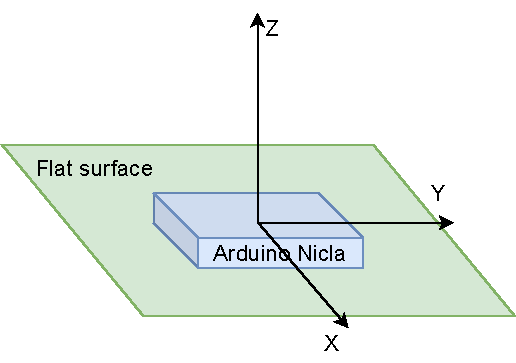
\includegraphics[width=.6\textwidth]{figures/Setup1and2}
        \caption{Setup used during the tasks: the sensor was placed in a flat surface with its $z$-axis pointing upwards
            (author's own work).}
        \label{fig:setup}
    \end{figure}


    \section{Results and Discussion}

    \subsection*{Task 1}

    The first task is intended to verify the performance of the magnetic sensor.
    The Nicla Sense ME Board was placed flat on a steady table and the magnetic field on the $x$, $y$ and $z$-axis were recorded.
    No drift is visible.
    The behaviour of all three axis are the same.
    Table~\ref{tab:magneticMeasurements} shows the offsets.
    Figure~\ref{fig:magneticFieldHist} shows the raw data together with the histogram of the raw data subtracted by the mean.

    \begin{figure}[h]

        \centering
        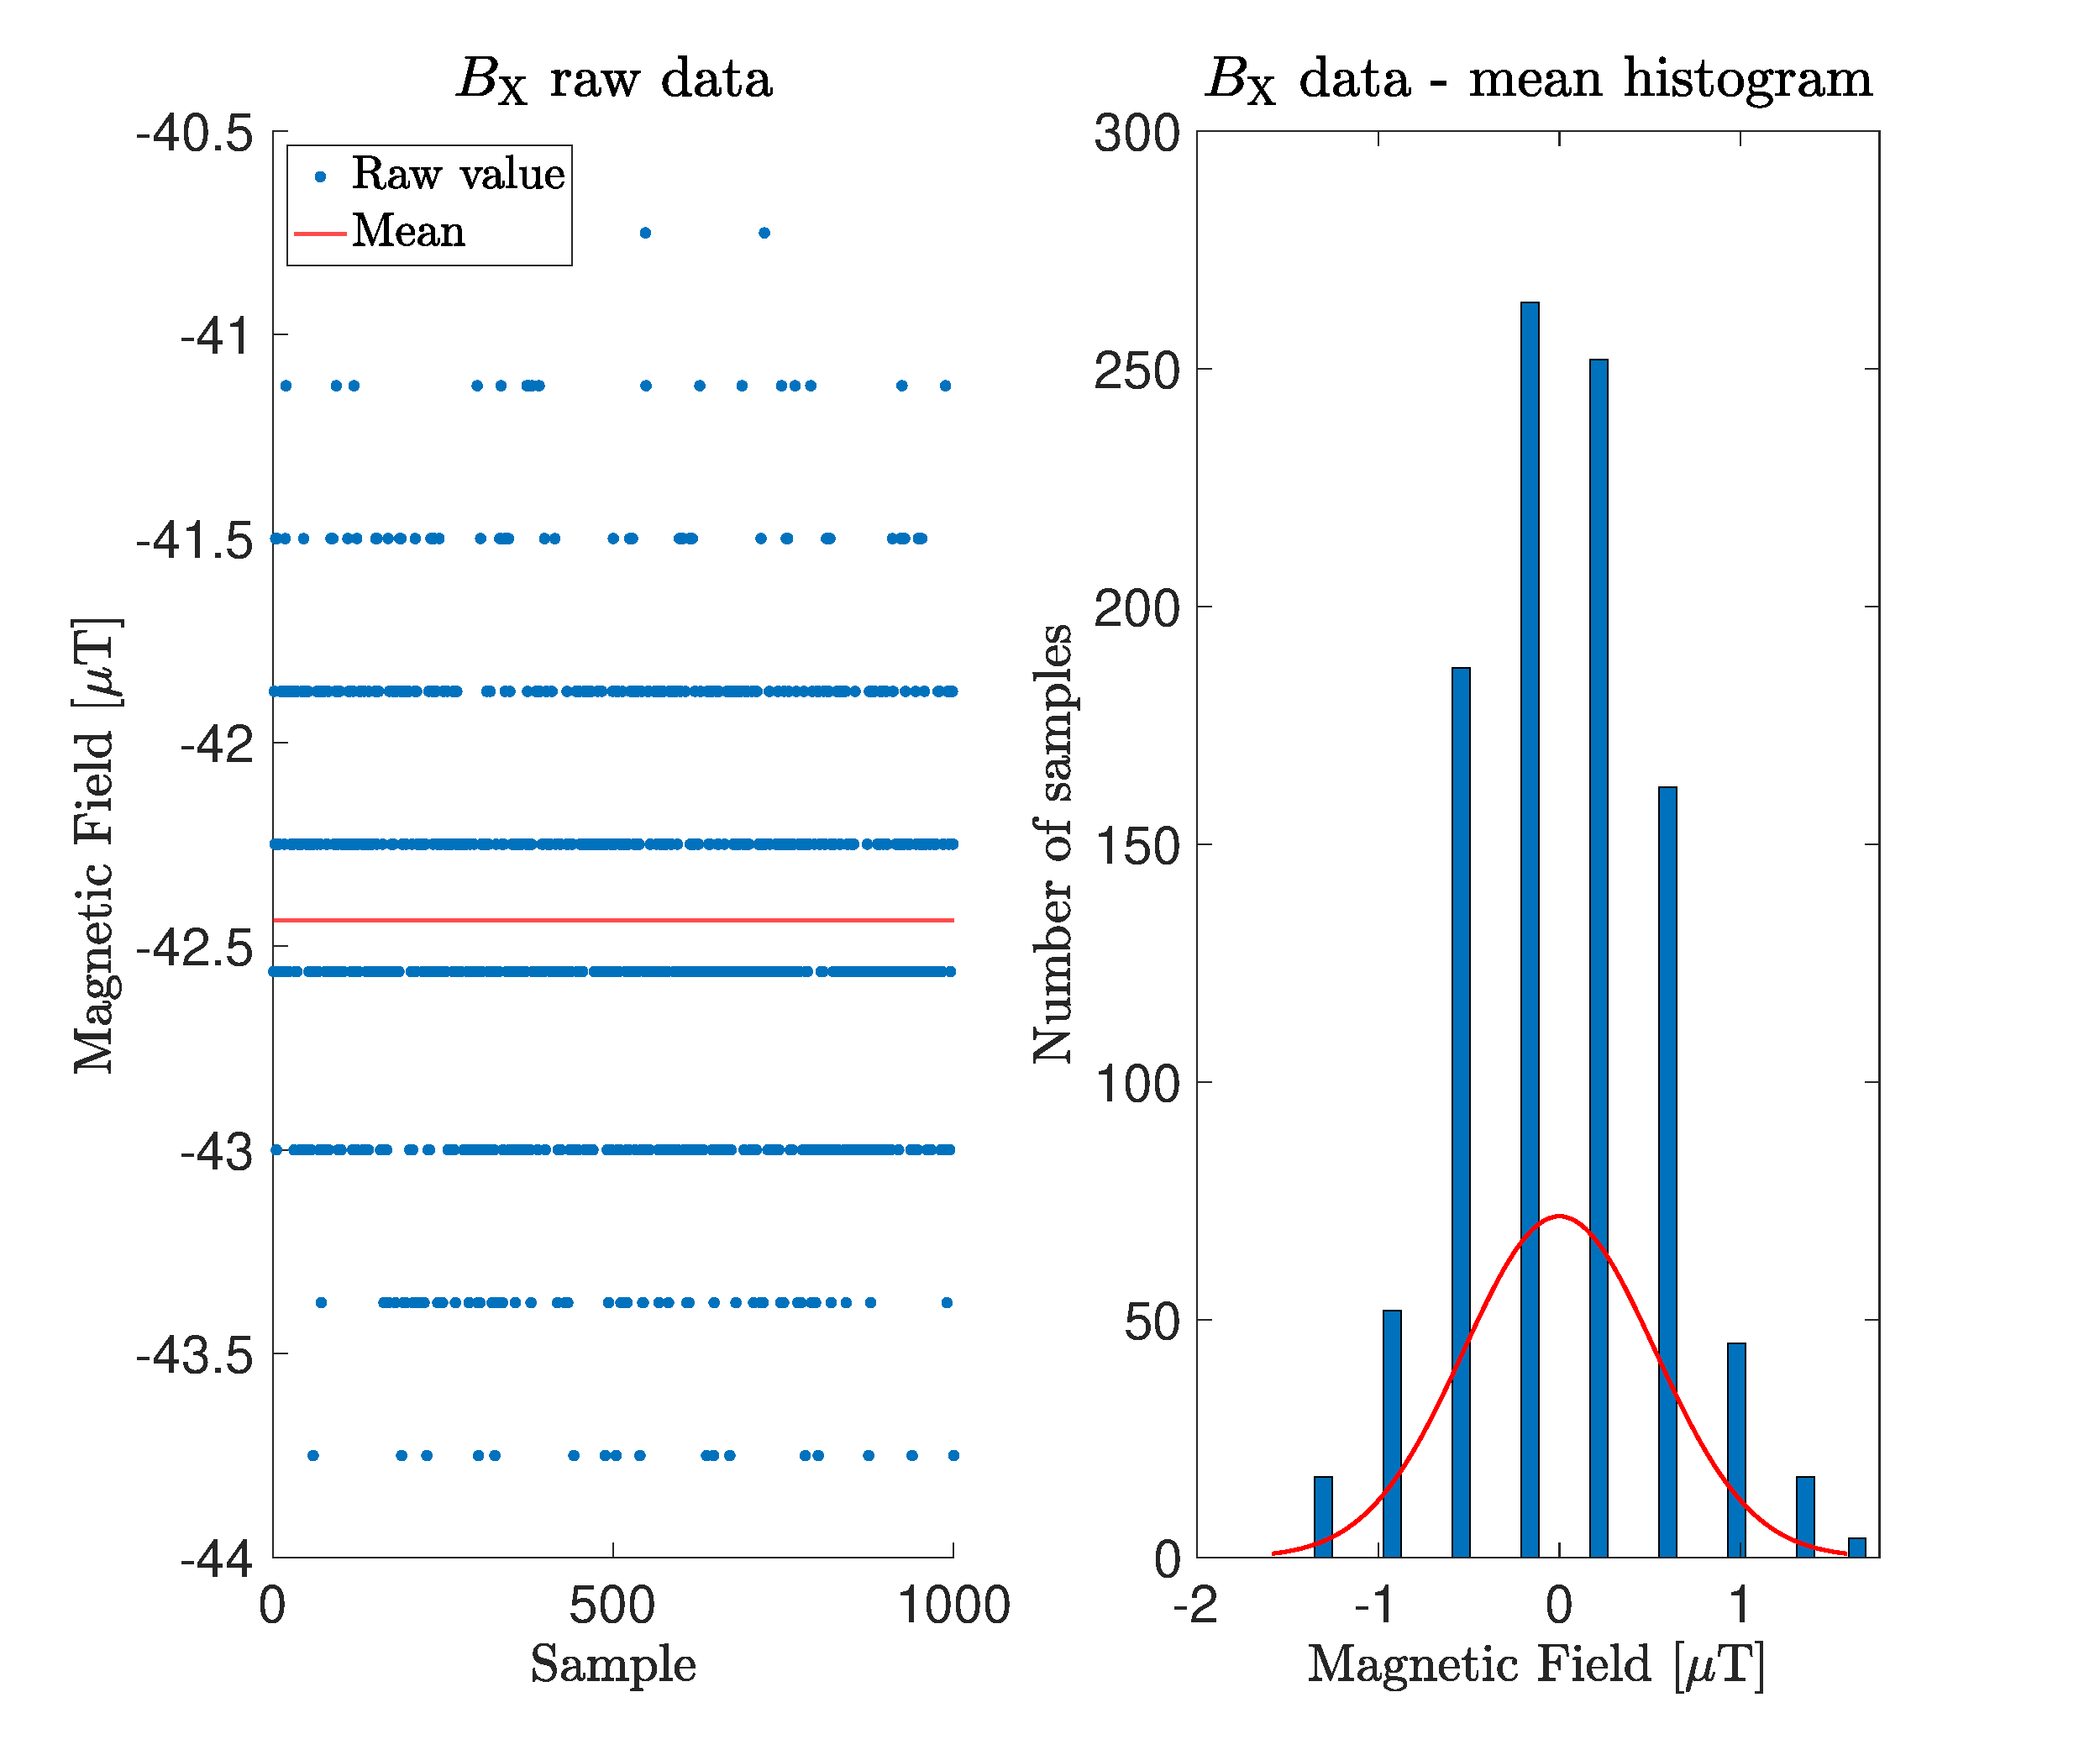
\includegraphics[width=.45\textwidth]{plots/plotMagFieldX}\hfill
        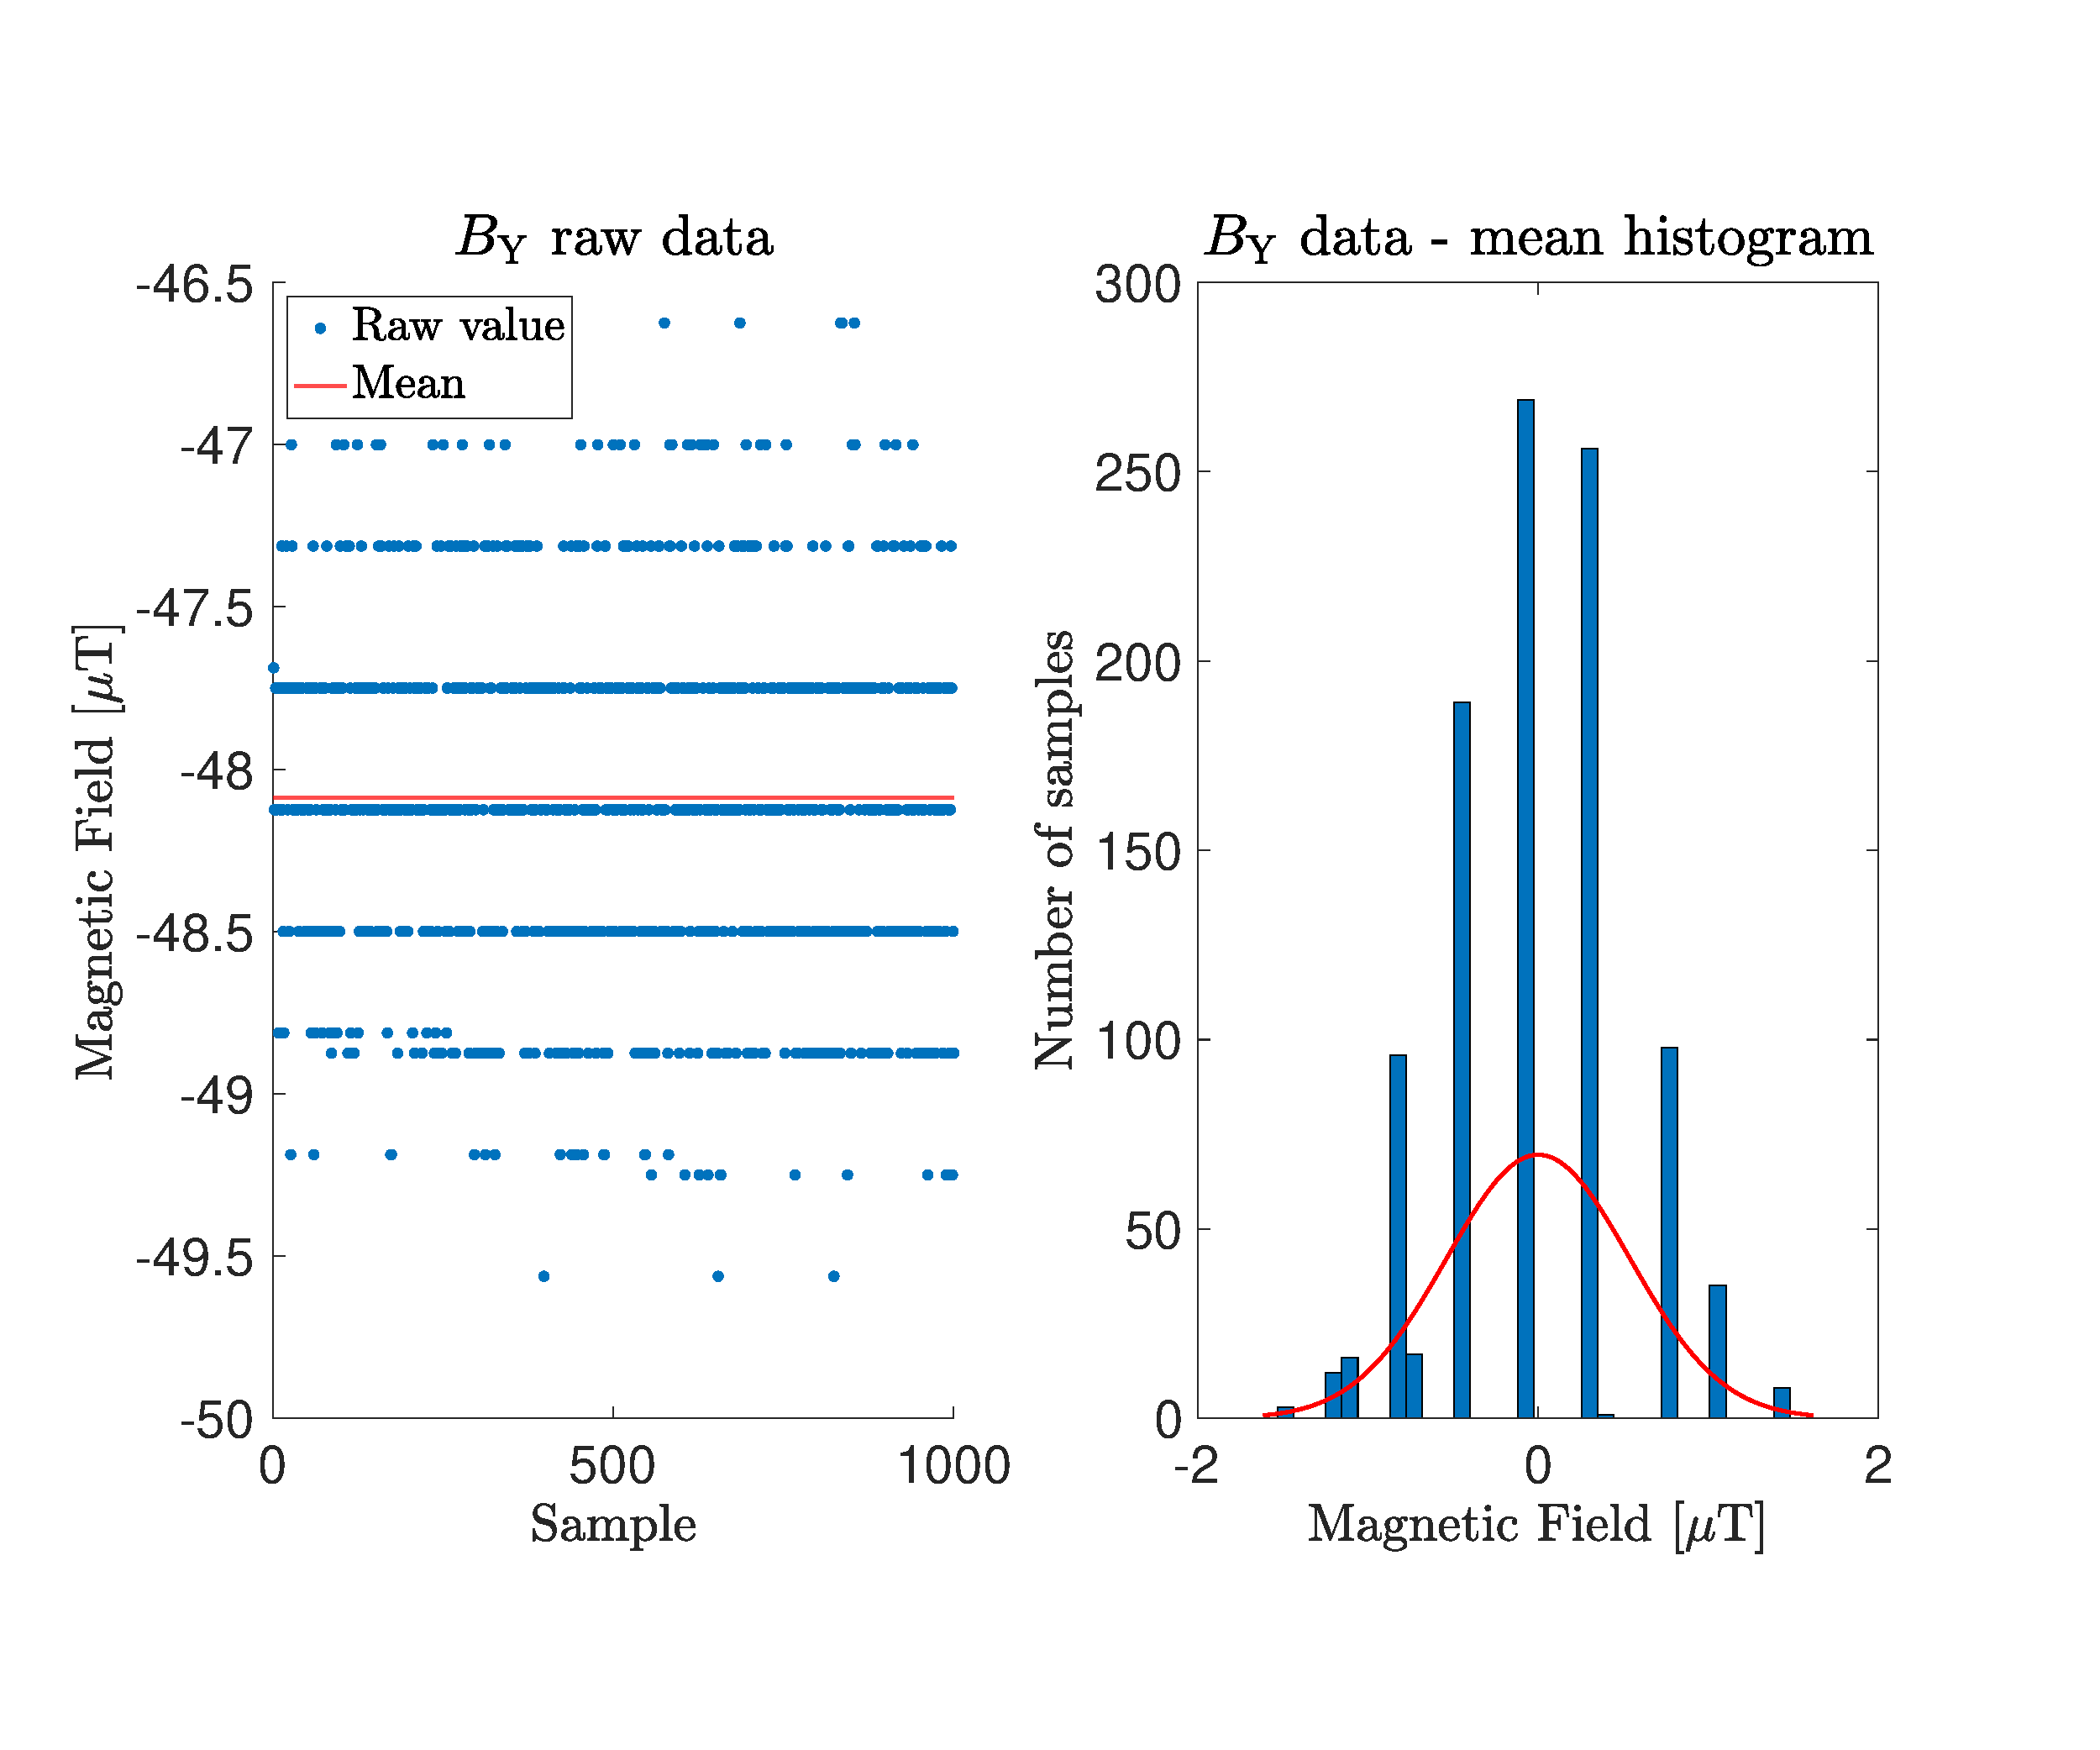
\includegraphics[width=.45\textwidth]{plots/plotMagFieldY}\vspace{1em}
        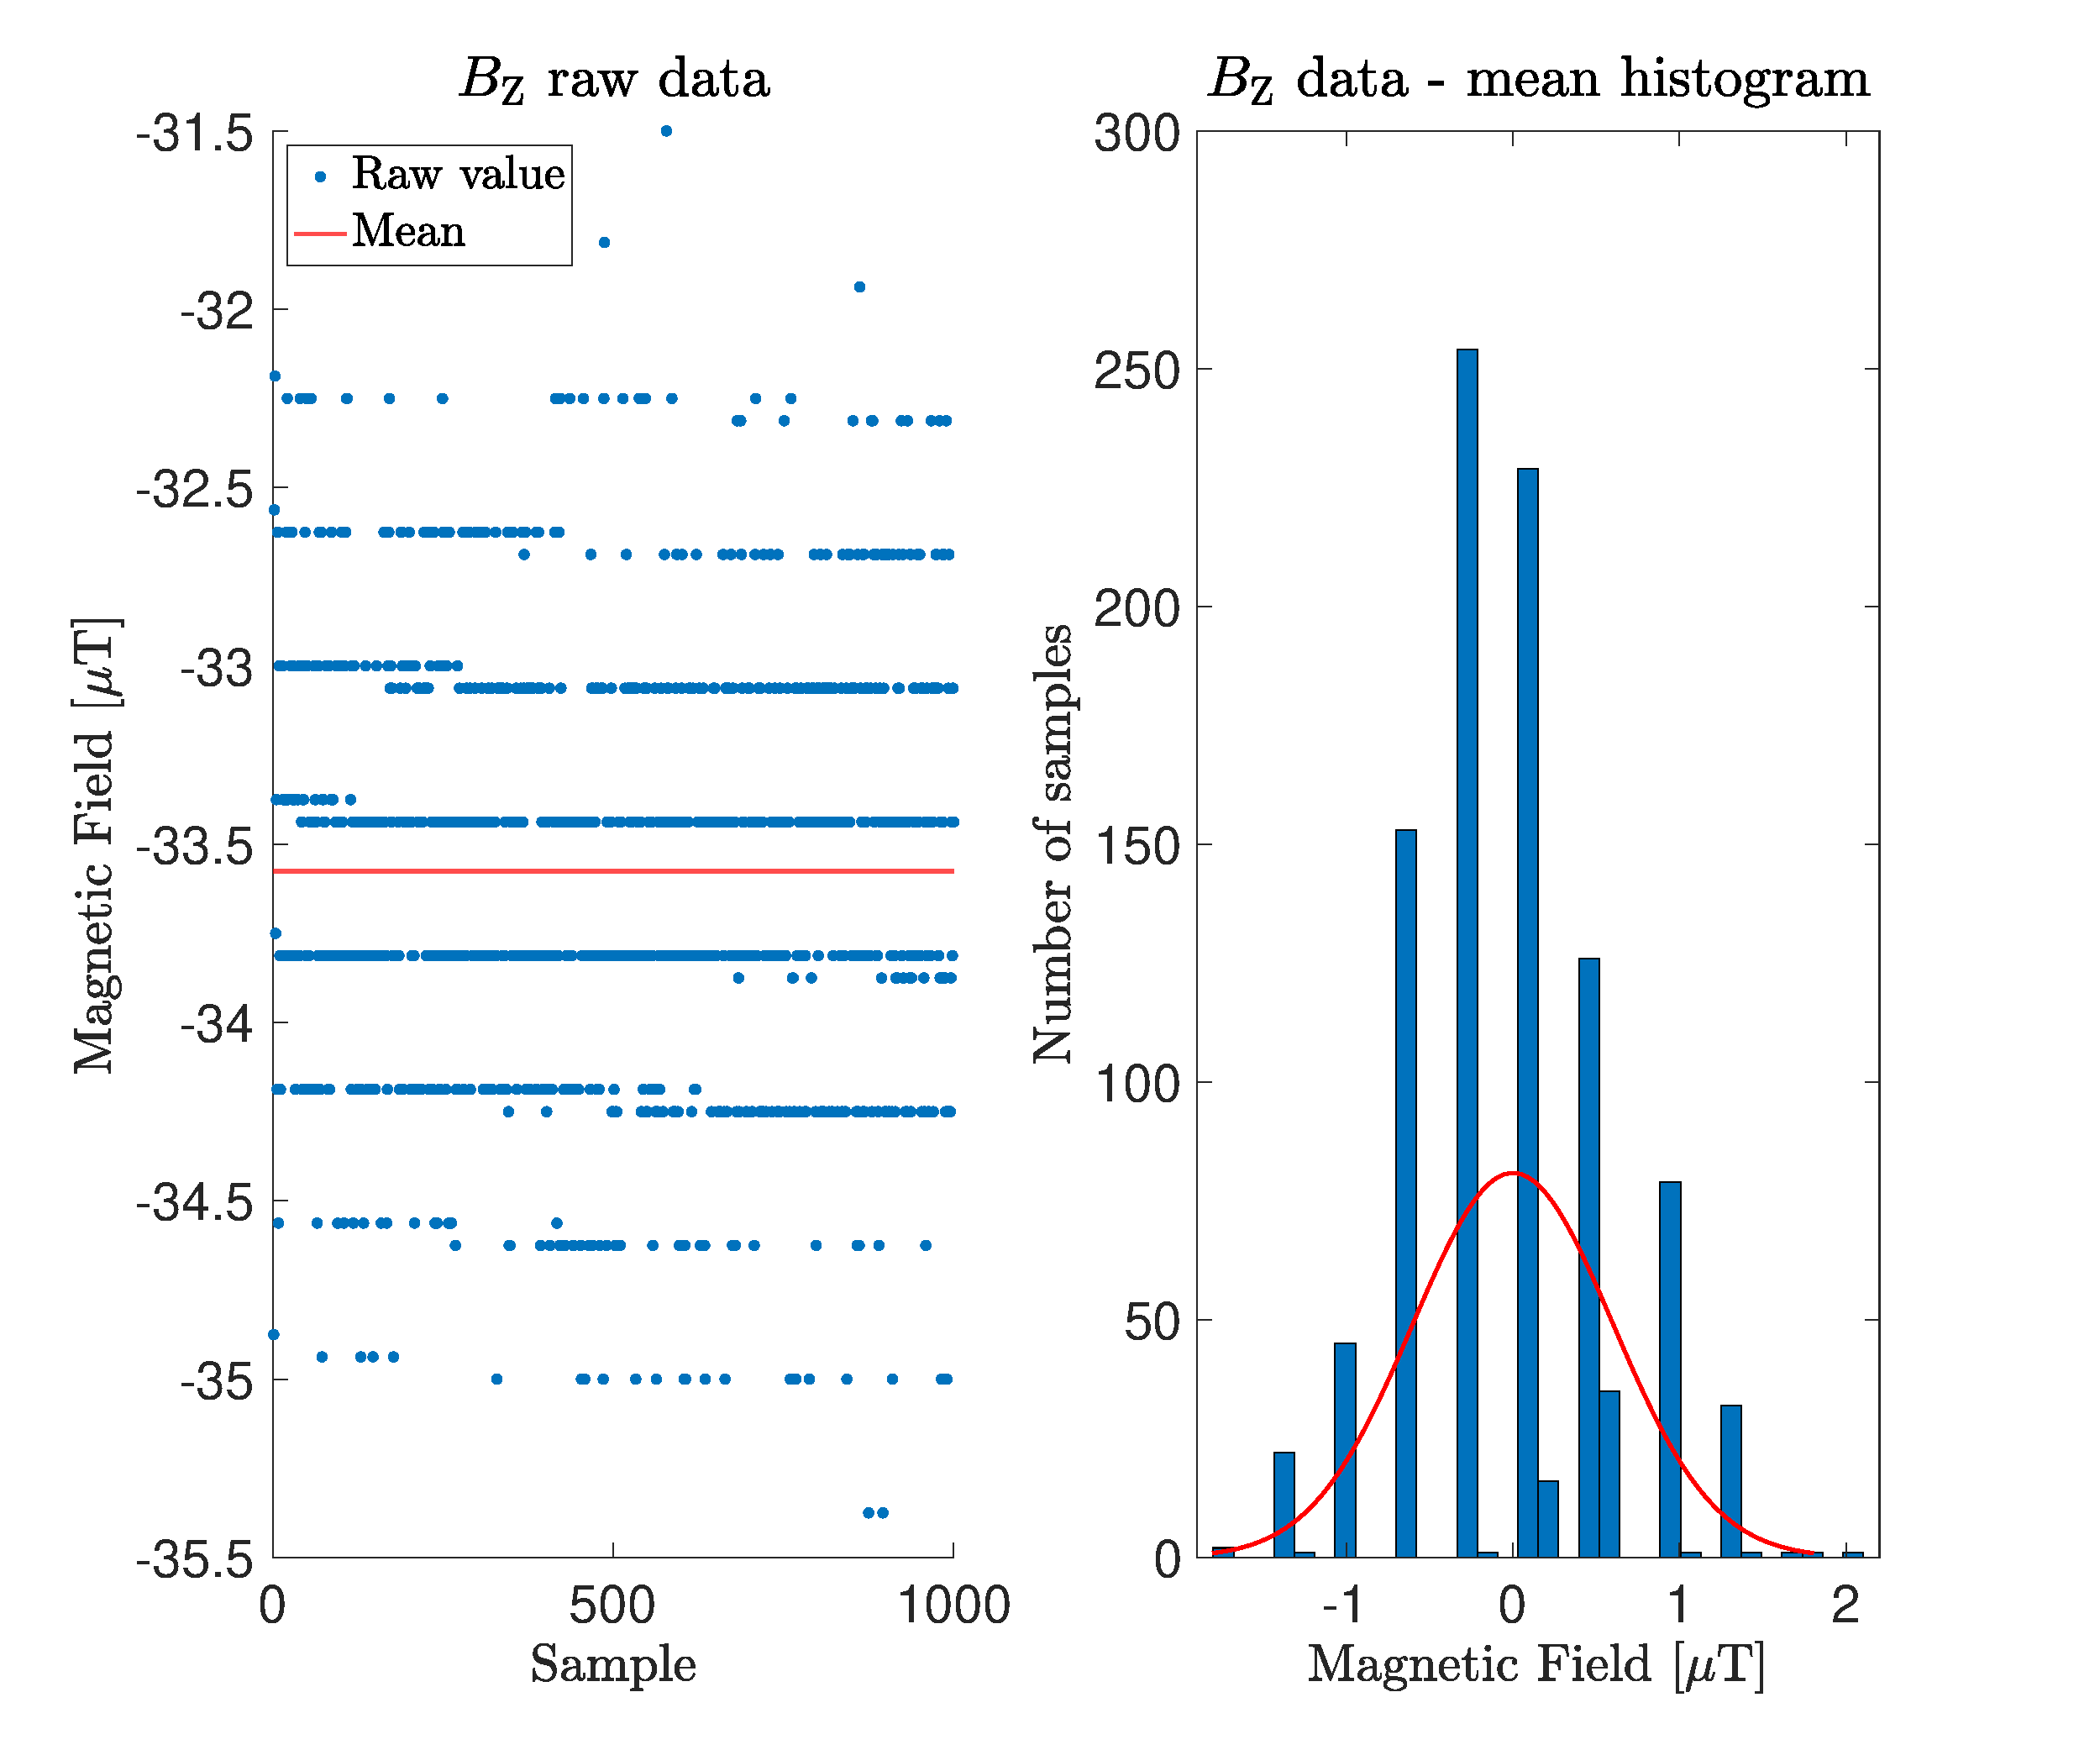
\includegraphics[width=.45\textwidth]{plots/plotMagFieldZ}\hfill
        \caption{Scatter raw data and histograms of the magnetic reading at rest with subtracted mean. All three directions allow approximation by a normal distribution.}
        \label{fig:magneticFieldHist}
    \end{figure}

    They follow a normal distribution with the mean ($\bar{\mathit{B}}$) and standard deviation($\sigma_B$) shown in Table~\ref{tab:magneticMeasurements}
    The $x$ and $y$-axis, which use the FlipCore technology, show slightly smaller standard deviation in comparison to the $z$-axis.

    \begin{table}[!ht]
        \centering
        \begin{tabular}{cS[table-format=1.3]S[table-format=1.3]S[table-format=1.3]}
            \hline \vspace{-1em} \\
            Direction & {$\bar{\mathit{B}}$ in \si{\micro\tesla}} & {$\sigma_B$ in \si{\micro\tesla}} \\ \hline
            $x$       & -42.43                                    & 0.5281                                         \\
            $y$       & -48.08                                    & 0.5385                                         \\
            $z$       & -33.57                                    & 0.6018                                         \\ \hline
        \end{tabular}
        \caption{Summary of the magnetic readings. The number of samples was 1,000 in each direction.
        Please note the quantization of \SI{0.0625}{\micro\tesla} for the individual values.}
        \label{tab:magneticMeasurements}
    \end{table}

    The results of Table~\ref{tab:magneticMeasurements} are consistent with the datasheet, since the standard deviation seen in
    the measurements is around $0.6\si{\micro\tesla}$ and the datasheet from BMM150 specifies a typical resolution
    of $0.3\si{\micro\tesla}$~\cite{BMM150} and a typical output noise of $0.6\si{\micro\tesla}$~\cite{BMM150}.


    \subsection*{Task 2}
    In task 2 we computed the offset of every axis of the sensors.
    The measurements were taken before and after flipping the sensor as specified in the section~\ref{sec:methods}.
    The non-flipped measurements were taken in the street along buildings 051 and 052 in the TF with the $y$-axis
    pointing the geographic north.
    Table~\ref{tab:offset} shows the results of the mean values before and after flipping, as well as the computed offset.

    \begin{table}[!ht]
        \centering
        \begin{tabular}{cS[table-format=1.3]S[table-format=1.3]S[table-format=1.3]}
            \hline \vspace{-1em} \\
            Direction & {$\bar{\mathit{B}}$ in \si{\micro\tesla}} & {$\bar{\mathit{B}}_{\mathrm{flipped}}$ in \si{\micro\tesla}} & {$\mathit{B}_{\mathrm{offset}}$ in \si{\micro\tesla}} \\ \hline
            $x$       & -39.43                                    & -47.73                                                       & -43.37 \\
            $y$       & -48.62                                    & 4.68                                                         & 26.65 \\
            $z$       & -21.10                                    & 102.65                                                       & 61.87 \\
        \end{tabular}
        \caption{Summary of the magnetic readings. The number of samples was 1,000 in each direction.
        Please note the quantization of \SI{0.0625}{\micro\tesla} for the individual values.}
        \label{tab:offset}
    \end{table}

    The datasheet specifies an offset of $40\si{\micro\tesla}$ in every direction~\cite{BMM150}.
    According to Table~\ref{tab:offset}, we can see that the values match with the specification, except the $z$-axis.
    A difference can be seen between the Hall sensor and FlipCore elements where the Hall sensor has a bigger offset
    as well as it is the only one outside the range of $40\si{\micro\tesla}$


    \subsection*{Task 3, 4}
    Task 3 was intended to measure the magnetic field outside, while task 4 to compute $B_{\mathrm{hor}}$, $B_{\mathrm{vert}}$ and $B$.
    Using the previously computed offsets the non-flipped data from task 2 was used for task 3 and 4.
    The mean value of the magnetic field for each axis, as well as its standard
    deviation were computed.
    They are shown in Table~\ref{tab:measurementOutside}

    \begin{table}[!ht]
        \centering
        \begin{tabular}{cS[table-format=1.3]S[table-format=1.3]S[table-format=1.3]}
            \hline \vspace{-1em} \\
            Direction & {$\bar{\mathit{B}}$ in \si{\micro\tesla}} & {$\sigma_B$ in \si{\micro\tesla}} \\ \hline
            $x$       & 3.936                                     & 0.547                             \\
            $y$       & 21.97                                     & 0.5385                            \\
            $z$       & -40.77                                    & 0.5255                            \\ \hline
        \end{tabular}
        \caption{Summary of the magnetic readings outside. The number of samples was 100 in each direction and the offset for
        each direction was subtracted.
        Please note the quantization of \SI{0.0625}{\micro\tesla} for the individual values.}
        \label{tab:measurementOutside}
    \end{table}

    Using the values from $B_x$, $B_y$ and $B_z$, $B_{\mathrm{hor}}$ and $B_{\mathrm{vert}}$ were computed using the
    equations~\ref{eq:Bhorizontal} and~\ref{eq:Bvertical} and compared with a model from~\cite{ngdc}.
    The latitude was 48.01366º N, longitude 7.83420º E and altitude 298.60\si{\meter} (GPS).
    The results are shown in Table~\ref{tab:measurementAndModel}.

    \begin{table}[!ht]
        \centering
        \begin{tabular}{cS[table-format=1.3]S[table-format=1.3]S[table-format=1.3]}
            \hline \vspace{-1em} \\
            Source           & {$B_{\mathrm{hor}}$ in \si{\micro\tesla}} & {$B_{\mathrm{vert}}$ in \si{\micro\tesla}} & {$B$ in \si{\micro\tesla}} \\ \hline
            Measurement      & 23.32                                     & -40.77                                     & 46.48                      \\
            WMM (2019-2024)  & 21.23                                     & 43.47                                      & 48.38                      \\ \hline
        \end{tabular}
        \caption{Comparison between of the magnetic readings outside and the model.}
        \label{tab:measurementAndModel}
    \end{table}

    The $z$-axis shows inverted signal, since the magnetic field is entering the earth.
    For the model this means a positive value and for the Arduino, it means a negative value as stated before in the section~\ref{sec:methods}.
    Because the $y$-axis was aligned to the geographic north, we can see that the $x$-axis measurement is quite small (in Table~\ref{tab:measurementOutside})
    compared to the other two axis.

    Considering the inverted $z$-axis, the difference between the model and the measurement, was 2.09 and 2.7\si{\micro\tesla} for both
    $B_{\mathrm{hor}}$ and $B_{\mathrm{vert}}$ respectively.
    Since the error in both is in the same range, one can also think that the reason is that the sensor was not perfectly
    perpendicular to the vertical and horizontal magnetic fields.
    The sensors output noise of $0.6\si{\micro\tesla}$ and resolution of $0.3\si{\micro\tesla}$ also add to the error.
    With that in mind we can say that the measurements are accurate.
    The total intensity $B$ is a result from $B_{\mathrm{hor}}$ and $B_{\mathrm{vert}}$ as shown in Equation~\ref{eq:Btotal},
    so the error of 1.9\si{\micro\tesla} makes sense.

    \subsection*{Task 5}
    Using the same dataset from task 3 and 4, on task 5 the angle of the magnetic north with respect to the
    geographic north, also known as declination, was computed.
    Since the $y$-axis was facing the geographic north, Equation~\ref{eq:magneticDeclination} was used.
    The results are shown in Table~\ref{tab:declination}.

    \begin{table}[!ht]
        \centering
        \begin{tabular}{cS[table-format=1.3]S[table-format=1.3]S[table-format=1.3]}
            \hline \vspace{-1em} \\
            Source           & {$B_x$ in \si{\micro\tesla}} & {$B_{y}$ in \si{\micro\tesla}} & {Declination in \si{\degree}} \\ \hline
            Measurement      & 3.93                         & 21.97                          & 10.15                         \\
            WMM (2019-2024)  & 1.14                         & 21.20                          & 3.08                          \\ \hline
        \end{tabular}
        \caption{Comparison between of the magnetic readings outside and the model.}
        \label{tab:declination}
    \end{table}

    Comparing the values, on $B_{y}$, we see an error of 0.77\si{\micro\tesla} which is almost within the noise range of the sensor.
    On the other hand, for $B_x$, an error of 2.79\si{\micro\tesla}, in which suggests that the sensor could have
    had a small inclination around the $y$-axis ($x$-axis not perpendicular to the magnetic field) when the measurement was taken.
    This could explain the 7º difference on the declination calculation.

    \section{Summary}
    Experiments show that the magnetic sensor readings are stable and displays no drift.
    The noise level is in the same range according to the specification of the sensor.
    The measurements and computations Earth's magnetic field are consistent to the model.



% BibTeX or Biber would be better options, with just 2 reference the "raw" approach is fine for such a report
    \begin{thebibliography}{------}

        \bibitem[1]{labManual} J. Kieninger, S.\,J. Rupitsch, \textit{Sensors Lab Course}.
        University Freiburg.
        Winter term 2022/23.
        \bibitem[2]{BMM150} \textit{BMM150 Datasheet}, Bosch Sensortec, BST-BMM150-DS001-05, rev. 1.4, April 2020.
        \bibitem[3]{CartographersOffice} \textit{Magnetic Declination – State Cartographer's Office – UW–Madison},
        Available: https://www.sco.wisc.edu/learning-center/magnetic-declination/. [Accessed: 03-Jan-2023]
        \bibitem[4]{fluxGate} \textit{How a fluxgate works}, Imperial College London,
        Available: https://www.imperial.ac.uk/space-and-atmospheric-physics/research/areas/space-magnetometer-laboratory/space-instrumentation-research/magnetometers/fluxgate-magnetometers/how-a-fluxgate-works/. [Accessed: 04-Jan-2023]
        \bibitem[5]{flixGateImage} https://popularelectronics.technicacuriosa.com/2017/03/16/inside-the-fluxgate-gradiometer/. [Accessed: 04-Jan-2023]
        \bibitem[6]{ngdc} https://www.ngdc.noaa.gov/geomag/calculators/magcalc.shtml#igrfwmm. [Accessed: 09-Jan-2023]
    \end{thebibliography}


\end{document}
